\chapter{The make Targets}
\label{app:tools}

Every step directory contains the same \cc{Makefile}, a link to
\cc{01_logic_gates/Makefile}. It expects the top module \cc{test} in
\cc{test.sv}, passes \emph{all} \cc{.sv} files of the directory to the tools,
and uses the testbench \cc{tb_test.cpp} and the pin file
\cc{../icebreaker.pcf}. All files it creates start with \cc{test}, except the
simulation files. \cc{make} without a target is \cc{make sim}.

\section{Overview}

\begin{center}
\small
\begin{tabular}{@{}>{\raggedright}p{20mm}>{\raggedright}p{56mm}>{\raggedright}p{24mm}>{\raggedright\arraybackslash}p{40mm}@{}}
\toprule
target & what it does & tools & creates \\
\midrule
\multicolumn{4}{@{}l}{\emph{Simulation}}\\
\cc{sim} & verilates, builds and runs the simulation (the default) & Verilator, C++ compiler & \cc{.stamp.verilate}, \cc{obj_dir/}, \cc{waveform.vcd} \\
\cc{verilate} & only translates the design to C++ & Verilator & \cc{.stamp.verilate}, \cc{obj_dir/} \\
\cc{build} & verilates and builds, but does not run & Verilator, C++ compiler & \cc{.stamp.verilate}, \cc{obj_dir/} \\
\cc{waves} & shows \cc{waveform.vcd} & GTKWave & \\
\cc{surfer} & shows \cc{waveform.vcd} & Surfer & \\
\cc{lint} & checks the SystemVerilog without simulating & Verilator & \\
\midrule
\multicolumn{4}{@{}l}{\emph{Synthesis and programming}}\\
\cc{test.v} & translates to Verilog & sv2v & \cc{test.v} \\
\cc{test.json} & synthesizes & yosys & \cc{test.json}, \cc{test.log} \\
\cc{test.asc} & places and routes & nextpnr & \cc{test.asc} \\
\cc{synth} & all of the above, then packs the bitstream & icepack & \cc{test.bin} \\
\cc{prog} & \cc{synth}, then writes the flash & iceprog & \\
\cc{gui-pnr} & nextpnr with its graphical interface & nextpnr & \\
\midrule
\multicolumn{4}{@{}l}{\emph{Looking at a design}}\\
\cc{svg}, \cc{png} & draws the circuit & yosys, netlistsvg, rsvg-convert & \cc{test_svg.json}, \cc{test.svg}, \cc{test.png} \\
\cc{report} & logic cells, Fmax, cells per module & nextpnr, yosys & \cc{test_report.txt}, \cc{test_report_pnr.log}, \cc{test_report_stat.txt} \\
\cc{floorplan} & where the design lies on the chip & nextpnr, Python 3 & \cc{test_pnr_dump.json}, \cc{test_floorplan.html} \\
\midrule
\cc{clean} & removes all of the files above & & \\
\bottomrule
\end{tabular}
\end{center}

\section{Simulation}

\textbf{\cc{make sim}} runs three stages, each printing a header
(Section~\ref{sec:step01-sim}):
\begin{description}
\item[VERILATING] runs
\begin{terminal}
verilator -Wall --trace --x-assign unique --x-initial unique -Wno-fatal
          -cc *.sv --top-module test --exe tb_test.cpp
\end{terminal}
  \cc{-Wall} turns on all warnings, \cc{-Wno-fatal} keeps them from stopping
  the build, \cc{--trace} adds the code that writes the VCD file. The other two
  options make Verilator give signals without a defined value (no initial value,
  no reset) a random value instead of 0, so that a design that relies on a
  value it never set is more likely to show it. The time stamp
  \cc{.stamp.verilate} records that this stage is done; it is repeated only
  when a \cc{.sv} file or the testbench changes.
\item[BUILDING SIM] compiles the generated C++ code with the testbench into
  the program \cc{obj_dir/Vtest}.
\item[SIMULATING] runs \cc{obj_dir/Vtest +verilator+rand+reset+2}, which
  chooses those random values at the start. The option reaches Verilator only
  if the testbench passes its command line on with
  \cc{Verilated::commandArgs(argc, argv);}, as the testbench of step 05 does;
  otherwise such signals start at 0. The testbench writes
  \cc{waveform.vcd}.
\end{description}
\textbf{\cc{make verilate}} stops after the first stage. \textbf{\cc{make
waves}} and \textbf{\cc{make surfer}} open \cc{waveform.vcd} in GTKWave or
Surfer, and run the simulation first if the file is missing.
\textbf{\cc{make lint}} runs \cc{verilator --lint-only}, a quick check of the
syntax and of the obvious errors, without \cc{-Wall} and without building
anything. \textbf{\cc{make build}} verilates and builds the program
\cc{obj_dir/Vtest} without running it.

\section{Synthesis and Programming}

The targets follow the tool flow of Figure~\ref{fig:toolflow}, each file made
from the previous one, and \cc{make} rebuilds only what is older than its
input:
\begin{terminal}
sv2v -v --define=SYNTHESIS --write=test.v *.sv
yosys -ql test.log -p 'synth_ice40 -abc9 -dffe_min_ce_use 4 -device u -dsp
      -top test -json test.json' test.v
nextpnr-ice40 --pcf-allow-unconstrained --up5k --package sg48 --json test.json
      --pcf ../icebreaker.pcf --asc test.asc
icepack test.asc test.bin
iceprog test.bin
\end{terminal}
The options of yosys: \cc{synth_ice40} is the complete synthesis for the
iCE40 family, \cc{-abc9} selects the newer logic optimizer, \cc{-device u} the
UltraPlus devices (our UP5K), \cc{-dsp} allows the multipliers (DSP blocks)
to be used, and \cc{-dffe_min_ce_use 4} uses the enable input of the
flip-flops only where at least four flip-flops share an enable
(Section~\ref{sec:step04-yosys}). The output goes to \cc{test.log}; its end
has the statistics we show in every chapter. nextpnr gets the device
(\cc{--up5k}, package \cc{sg48}) and the pin file, and
\cc{--pcf-allow-unconstrained} turns a missing pin into a warning instead of an
error (Section~\ref{sec:step02-pins}). nextpnr prints its report, with the
utilisation and the maximal frequency, to the terminal.

\textbf{\cc{make synth}} produces \cc{test.bin}, \textbf{\cc{make prog}}
also writes it into the flash of the board.

\subsection*{make gui-pnr}

runs nextpnr with the same options and \cc{--gui}. A window opens with the
chip and the netlist loaded, and nothing done yet. The buttons \emph{Pack},
\emph{Place} and \emph{Route} in the toolbar run the three phases of nextpnr
one at a time, so you can watch the logic cells appear on the chip during
placement and the wires during routing, and click on a cell or a wire to see
what it is. For small designs like step 01 or 02 this is the best way to see
what place and route means. Build the bitstream for the board with
\cc{make synth}, not here.

\section{Pictures of a Design}

\textbf{\cc{make svg}} runs yosys with \cc{prep -top test} instead of
\cc{synth_ice40}, so the netlist keeps the gates, adders, multiplexers and
flip-flops as we wrote them, and keeps submodules as boxes. netlistsvg draws
this netlist as \cc{test.svg}. \textbf{\cc{make png}} converts it into
\cc{test.png}, 2000 pixels high. Figures~\ref{fig:step01-netlist},
\ref{fig:step02-netlist} and~\ref{fig:step03-netlist} were made this way. From
step 05 on, the pictures become too large to read.

\section{make report}
\label{sec:tools-report}

\cc{make report} prints a summary of the resources a design uses. It runs
nextpnr once more, without writing a bitstream, and keeps its log in
\cc{test_report_pnr.log}. Then it runs yosys a second time with
\cc{synth_ice40 -noflatten}, which keeps the modules apart, and keeps the
statistics in \cc{test_report_stat.txt}. From both it writes
\cc{test_report.txt} and prints it. For the ULM of step 09:

\outputfile{tools_report.txt}

The first part is the utilisation reported by nextpnr, without the resources
the design does not use: logic cells, block RAMs (\cc{ICESTORM_RAM}), I/O pins,
global buffers for clocks (\cc{SB_GB}), DSP blocks and the large single-port
RAMs (\cc{ICESTORM_SPRAM}). Then the maximal clock frequency of the final
placement, and if the design has no clock, a line saying so.

The second part comes from the non-flattened synthesis. Its first line is the
whole design, \cc{test} with everything in it. Every line below counts the cells
of one submodule \emph{itself}, without its own submodules, which are indented
under it: \cc{uart_rx} has 65 cells of its own, and its \cc{baud_tick_gen} 58
more. These are cells before packing (a LUT and a flip-flop that later share
one logic cell count as two), so the numbers are larger than the logic cells of
the first part. Two more things to know. A module whose ports are interfaces
(Chapter~\ref{ch:step07}) does not appear: sv2v merges it into its parent, so
its cells are counted with the parent, here with \cc{test}. And each module is
listed once, with the cells of one instance, even if it has several instances:
\cc{dp_bram4096} is used twice in the ULM. yosys names modules with parameters
\cc{$paramod$...}; the report strips that prefix.

\section{make floorplan}
\label{sec:tools-floorplan}

\cc{make floorplan} shows where the design ends up on the chip. It runs
nextpnr with the option \cc{--post-route tools/pnr_dump.py}. nextpnr has a
Python interpreter built in, and after routing it runs this script, which
writes every site of the chip (every logic cell, block RAM, I/O pin, \dots)
with its position and the name of the cell placed there into
\cc{test_pnr_dump.json}. The script \cc{tools/floorplan.py} turns this into
the page \cc{test_floorplan.html}, and on a Mac, \cc{make} opens it in the
browser. The page shows three things:
\begin{itemize}
\item \textbf{The chip.} Each square is a logic tile with its eight logic
  cells, drawn as eight thin bars, colored by the top-level instance a cell
  belongs to; free cells are grey. The tall boxes are block RAMs and DSPs,
  the small squares SPRAMs and I/O pins, dashed if unused. Hovering over a
  tile lists what is in it.
\item \textbf{A treemap.} One rectangle per top-level instance, with an area
  proportional to its number of logic cells, divided into its sub-instances.
\item \textbf{A table} with the same numbers, the blocks each instance uses
  (block RAMs, DSPs, SPRAMs, I/O pins), and its largest parts.
\end{itemize}
The seven largest instances get a color of their own, the rest is shown as
``Other''. Figure~\ref{fig:tools-floorplan} shows the chip for step 09.

\begin{figure}[ht]
\centering
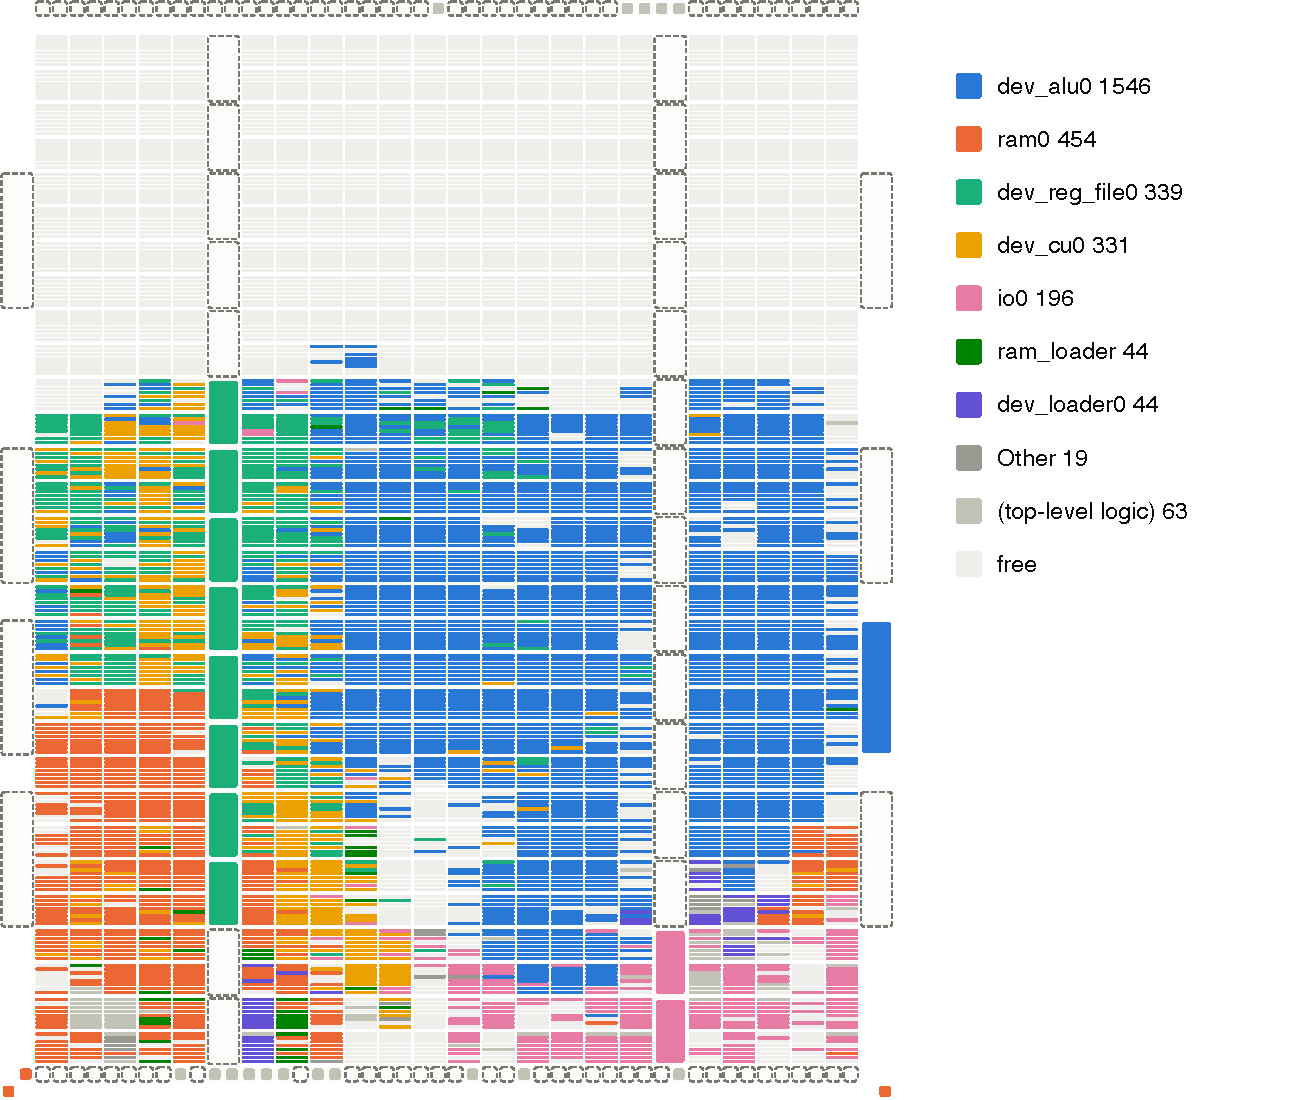
\includegraphics[width=0.85\linewidth]{figures/tools_floorplan.pdf}
\caption{The chip view of \cc{make floorplan} for step 09, with the number of
logic cells per top-level instance. The block RAMs of the register file
(\cc{dev_reg_file0}) form a column in the left half; the DSP used by the ALU
is the box on the right edge.}
\label{fig:tools-floorplan}
\end{figure}

\begin{pitfall}
The page knows only the names of the cells. yosys names a cell after the
net it drives, and after flattening this name begins with the instance path,
like \cc{dev_hex0.counter[3]} in Section~\ref{sec:step03-yosys}. The page
counts a cell for the instance at the beginning of its name. This is a good
approximation, but a cell at the boundary between two modules, for instance a
LUT that computes an input of one module from outputs of another, may be
named after the other module and be counted there. Cells whose names have no
instance path, and the extra cells nextpnr adds itself, appear as
``(top-level logic)''. So the numbers of the page and of \cc{make report}
differ a little.
\end{pitfall}

\section{make clean}

\cc{make clean} removes everything the Makefile creates: \cc{.stamp.*},
\cc{obj_dir}, \cc{waveform.vcd}, \cc{test.v}, the files of synthesis, place
and route and programming, the pictures, the report and the floorplan. The
sources (\cc{*.sv}, \cc{tb_test.cpp}) are never touched.
